\documentclass{beamer}


%----------------------- Preamble ----------------

\usepackage[T1]{fontenc}	%Fremmedord
\usepackage[utf8]{inputenc} %Input type
\usepackage[danish]{babel}	%sprog
\usepackage{lmodern}		%Dansk skriftpakke
\hypersetup{pdfstartview={Fit}}

%Standard sti at søge efter billeder
%--------------------------------------------------
%\begin{figure}[hbtp]
%\centering
%\includegraphics[scale=1]{filnavn-for-png}
%\caption{Titel}
%\label{fig:referenceNavn}
%\end{figure}
%--------------------------------------------------
\usepackage{graphicx}
\usepackage{float}
\graphicspath{{Figurer/}}


%Speciel skrift for enkelt linje kode
%--------------------------------------------------
%Udskriver med fonten 'Courier'
%Mere info her: http://tex.stackexchange.com/questions/25249/how-do-i-use-a-particular-font-for-a-small-section-of-text-in-my-document
%Eksempel: Funktionen \code{void Hello()} giver et output
%--------------------------------------------------
\newcommand{\code}[1]{{\fontfamily{pcr}\selectfont #1}}

%Tables
%----------------------------------------------------------
\usepackage{tabularx}
\usepackage{multirow} 
\usepackage{multicol} 
\usepackage{booktabs}


% Følgende er til koder.
%----------------------------------------------------------
%\begin{lstlisting}[caption=Overskrift på boks, style=Code-C++, label=lst:referenceLabel]
%public void hello(){}
%\end{lstlisting}
%----------------------------------------------------------

%Exstra space
\usepackage{xspace}
%Navn på bokse efterfulgt af \xspace (hvis det skal være mellemrum
%gives det med denne udvidelse. Ellers ingen mellemrum.
\newcommand{\codeTitle}{Code snippet\xspace}

%Pakker der skal bruges til lstlisting
\usepackage{listings}
\usepackage{color}
\usepackage{textcomp}
\definecolor{listinggray}{gray}{0.9}
\definecolor{lbcolor}{rgb}{0.9,0.9,0.9}
\renewcommand{\lstlistingname}{\codeTitle}
\lstdefinestyle{Code}
{
	keywordstyle	= \bfseries\ttfamily\color[rgb]{0,0,1},
	identifierstyle	= \ttfamily,
	commentstyle	= \color[rgb]{0.133,0.545,0.133},
	stringstyle		= \ttfamily\color[rgb]{0.627,0.126,0.941},
	showstringspaces= false,
	basicstyle		= \small,
	numberstyle		= \footnotesize,
%	numbers			= left, % Tal? Udkommenter hvis ikke
	stepnumber		= 2,
	numbersep		= 6pt,
	tabsize			= 2,
	breaklines		= true,
	prebreak 		= \raisebox{0ex}[0ex][0ex]{\ensuremath{\hookleftarrow}},
	breakatwhitespace= false,
%	aboveskip		= {1.5\baselineskip},
  	columns			= fixed,
  	upquote			= true,
  	extendedchars	= true,
 	backgroundcolor = \color{lbcolor},
	lineskip		= 1pt,
%	xleftmargin		= 17pt,
%	framexleftmargin= 17pt,
	framexrightmargin	= 0pt, %6pt
%	framexbottommargin	= 4pt,
}

%Bredde der bruges til indryk
%Den skal være 6 pt mindre
\usepackage{calc}
\newlength{\mywidth}
\setlength{\mywidth}{\textwidth-6pt}


% Forskellige styles for forskellige kodetyper
\usepackage{caption}
\DeclareCaptionFont{white}{\color{white}}
\DeclareCaptionFormat{listing}%
{\colorbox[cmyk]{0.43, 0.35, 0.35,0.35}{\parbox{\mywidth}{\hspace{5pt}#1#2#3}}}
\captionsetup[lstlisting]
{
	format			= listing,
	labelfont		= white,
	textfont		= white, 
	singlelinecheck	= false, 
	width			= \mywidth,
	margin			= 0pt, 
	font			= {bf,footnotesize}
}

\lstdefinestyle{Code-Java} {language=Java, style=Code}


\title{ITONK eksamen}
\subtitle{RMI}

\author % (optional, for multiple authors)
{Rasmus Bækgaard\inst{1}}

\institute%[Universitäten Hier und Dort] % (optional)
{
  \inst{1}%
  Information og Kommunikationsteknologi\\
  Ingeniørhøjskolen i Aarhus
}

\date{\today}

\subject{subject\dots}

%----------------------- Preamble ----------------

\begin{document}

	\frame{\titlepage}
	
%\AtBeginSection[]
%{
	\begin{frame}
		\frametitle{Table of content}
		\tableofcontents%[currentsection, currentsubsection]
	\end{frame}
%}

\section{The purpose of RMI}
	\begin{frame}
		\frametitle{What is the purpose of RMI?}
		
		\begin{itemize}
		\item Remote Method Invocation -- RMI
		\item Java Virtual Machine -- JVM
		\item Access to other clients objects
		
			\begin{itemize}
			\item Distribute tasks
			\end{itemize}
		\end{itemize}
			
	\end{frame}
	
	
	
\section{The three main layers in the RMI architecture}
	\begin{frame}
		\frametitle{The three main layers in the RMI architecture}
		
		\begin{itemize}
		\item Stub and Skeleton Layer -- Interface
		\item Remote Reference Layer -- Serialize and TCP/IP
		\item Transport Layer
		\end{itemize}
		
		\begin{figure}[hbtp]
		\centering
		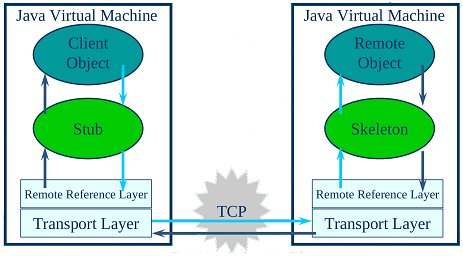
\includegraphics[scale=0.7]{JVM}
		\end{figure}		

				
	\end{frame}
		

\section{The RMI Registry}
	\begin{frame}
		\frametitle{The RMI Registry}
		
		\begin{itemize}
		\item Traditionally RMI Registry keeps all server
		\item Servers link to Clients
		\item Uses Port and IP
		\end{itemize}
		
		\begin{figure}[H]
			\begin{minipage}[b]{0.5\linewidth}
			\centering
			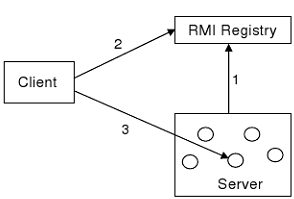
\includegraphics[width=\linewidth]{RMI-registry}
			\end{minipage}			
			\hspace{0.5cm}
			\begin{minipage}[b]{0.4\linewidth}
			\centering
			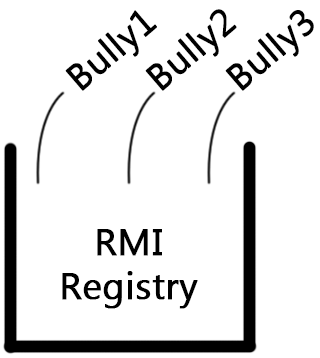
\includegraphics[width=\linewidth]{RMI-reg}
			\end{minipage}
		\end{figure}
				
	\end{frame}
	
	
\section{The remote interface}
	\begin{frame}[fragile]
		\frametitle{The remote interface}

		\begin{lstlisting}[caption=Remote interface, style=Code-Java]
		public interface Bully extends Remote {
			String DoTask() throws RemoteException;
			void StartElection() throws RemoteException;
			void Announce(ClientDTO newLeader) throws RemoteException;
		}
		\end{lstlisting}
		
		
		\begin{lstlisting}[caption=Call client, style=Code-Java]
		Registry reg = LocateRegistry.getRegistry(client.host, client.port);
						Bully skeleton = (Bully) reg.lookup("Bully1");
		\end{lstlisting}
	
	\end{frame}
	

\section{Leader election, and Bully Election}
	\begin{frame}
		\frametitle{Leader election, and Bully Election}
		
		\begin{itemize}
		\item Leader / coordinator manages task for clients
		\item Bully election
		\item Big-O($N^2$)
		\item Static list of members
		\end{itemize}
		
		\begin{figure}[hbtp]
		\centering
		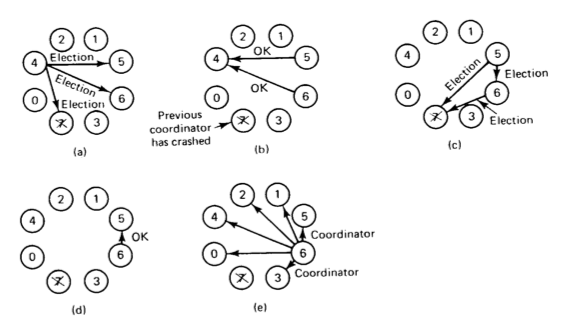
\includegraphics[scale=0.5]{BullyAlgorithm}
		\end{figure}		
				
	\end{frame}
	
\subsection{Improving Bully Election}
	\begin{frame}
		\frametitle{Improving Bully Election}
		
		\begin{itemize}
		\item Reduce amount of messages
		\item Know one -- connect to all
		\item Adding: Big-O($2+3N$)
		
			\begin{itemize}
			\item Add me
			\item Stop for election
			\item Elect me
			\end{itemize}
		
		\end{itemize}
		
		\begin{figure}[hbtp]
		\centering
		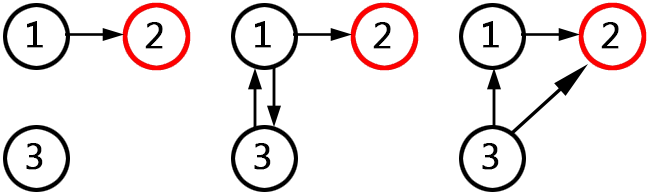
\includegraphics[scale=0.4]{RMI-Smart-Election}
		\end{figure}		

	\end{frame}

\end{document}